\documentclass[conference]{IEEEtran}
\usepackage[T1]{fontenc}
\usepackage{graphicx}
\usepackage{booktabs}
\usepackage{amsmath}
\usepackage{url}

\begin{document}

\title{Blind Noise-Template Subtraction with a Fine-Tuned Demucs Denoiser for Indic Speech Noise Removal}

\author{\IEEEauthorblockN{Saifuddin}
\IEEEauthorblockA{Team syehsyoh; Senior Digital Transformation (AI \& Automation) Expert\\
Datathon@IndoML 2026, Track 2 (Noise Event Removal)\\
Code, checkpoints and templates: \url{https://github.com/syehsyoh-dokling/NoiseRemoval}}}

\maketitle

\begin{abstract}
Track~2 asks for Vaani speech recordings with their noise events removed, scored by SI\nobreakdash-SDR on synthetic
clips plus the change in word error rate of a mandated ASR. Our submission (Codabench 995100) placed 2nd on the
Phase\nobreakdash-2 leaderboard with a combined score of 21.2379 (SI\nobreakdash-SDR 16.770\,dB,
$\Delta$WER$\times$100 4.468, audit passed). It rests on one observation: the synthetic test clips reuse a library of
noise waveforms that, by our evidence, is not the validation library.
We discover those waveforms blindly from the residual of a denoiser, subtract the detected copies with a least-squares
gain, and run a Demucs denoiser fine-tuned with an SI\nobreakdash-SDR loss restricted to event-free target samples on
what remains. Template subtraction followed by re-denoising added 8.48 points over the denoiser-only system
(12.7544 to 21.2379).
\end{abstract}

\section{Training Data and Preprocessing}
\textbf{Vaani data.} We used the released validation set of Track~2: 695 synthetic clips (noisy mixture, clean
reference and noise timestamps) and 1,806 natural noisy clips, all 16\,kHz mono. We also used the Gold tier of the
Vaani noise-event dataset~\cite{vaani}: 10,772 clips with verified noise-event timestamps. The Phase\nobreakdash-2 test set holds
3,178 unlabelled clips. No clean references or timestamps of the test set were accessed. Beyond the test audio
itself, which template discovery consumes transductively (Sec.~\ref{sec:tpl}), two pieces of test-side information
were used: (a)~the leaderboard score of each of our Phase\nobreakdash-2 submissions, the model-selection criterion
(Sec.~\ref{sec:res}); (b)~Codabench's per-clip result page, which lists per-clip SI\nobreakdash-SDR for 500 synthetic
test clips of its own choosing (it reports the split as 1,099 synthetic, 2,079 natural), used for the per-clip
analyses in Sec.~\ref{sec:res} including the ESC-50 decision. Discovery ran on all 3,178 clips without that split.

\textbf{Noise bank.} A synthetic clip is its clean reference plus pasted noise, up to quantisation (outside the
pasted spans the residual is about $10^{-4}$ in amplitude, full scale 1), so mixture minus reference gives 2,213
noise snippets, the only noise source used for training augmentation in the final system.

\textbf{Augmentation pipeline.} Training mixtures are made on the fly. (1)~A target recording is drawn; of four random
4\,s crops the one with the largest event-free share is kept (redrawn if below 30\%). (2)~With probability 0.85,
1--3 bank snippets are pasted at random positions. (3)~Each snippet's RMS relative to the local target RMS follows a
log-normal law centred on the median ratio of the validation mixtures ($\sigma=0.5$ in natural-log units).
(4)~Mixture and target are jointly peak-limited to 0.99. Targets are the 1,806 natural validation clips and the Gold
clips; the 695 clean references are added as targets from stage~1 on (Sec.~\ref{sec:den}).

\textbf{Event-free masks.} Natural and Gold recordings almost always contain real noise events (99.9\% of clips; mean
coverage 27--30\%). Each target gets a mask that is 0 inside annotated events dilated by $\pm$150\,ms and 1
elsewhere; clean references are fully 1.

\textbf{Local validation.} Early variants were compared on 200 held-out synthetic validation clips, at the validation
SNR and remixed at the test-like SNR. From stage~0 on every validation clip enters training (natural clips as
targets, synthetic clips through the bank, clean references as targets from stage~1), so no held-out set remained;
moreover the test noise differs from the validation noise (Sec.~\ref{sec:tpl}): the clean-reference variant that won
on both held-out sets (mean SI\nobreakdash-SDR 23.30 vs.\ 18.18\,dB, test-like SNR) lost on the leaderboard
(Table~\ref{tab:abl}, row~3). Later comparisons therefore used leaderboard submissions.

\textbf{Additional datasets.} ESC-50~\cite{esc50} was tested as extra bank noise in one rejected variant (12.0588
vs.\ 12.3660 without it); it is not used by the final system.

\section{Proposed Method}
\subsection{Background}
SI\nobreakdash-SDR~\cite{sisdr} projects the estimate onto the reference, so it is gain-invariant; it is
$-\mathcal{L}$ in (1) with $m\equiv1$. The combined score is the mean SI\nobreakdash-SDR over the 1,099 synthetic
clips plus $\Delta$WER$\times$100, with $\Delta$WER $=$ WER(noisy) $-$ WER(enhanced) pooled over the words of all
3,178 clips (WER: word edits over reference words). Demucs~\cite{demucs} is a waveform-domain U-Net with an LSTM
bottleneck; its dns64 weights, trained on DNS-challenge data~\cite{dns}, are our starting point. Template subtraction
rests on the matched filter~\cite{turin}: for a known waveform $T$ in additive white noise the correlator
$\langle x,T\rangle$ is the optimal detector, and normalised cross-correlation~\cite{lewis} makes it gain-invariant.
The least-squares gain $g=\langle x,T\rangle/\lVert T\rVert^2$ is the projection of the mixture onto $T$, so $x-gT$
removes an exact copy up to the bias $\langle s,T\rangle/\lVert T\rVert^2$ that the speech induces in $g$;
repeating the search on the residual (pass~2) is a batched form of matching pursuit~\cite{mallat}. Unlike
REPET~\cite{repet}, which exploits repetition within one recording, the dictionary here is built across clips from a
denoiser's residuals.

\subsection{Denoiser}\label{sec:den}
The denoiser is Demucs in the dns64 configuration~\cite{demucs} (causal U-Net encoder/decoder with an LSTM bottleneck,
hidden size 64, 16\,kHz), initialised from the public pretrained dns64 weights~\cite{denoiserrepo}. The loss is the
negative SI\nobreakdash-SDR~\cite{sisdr} computed only where the event-free mask $m$ of the target $s$ is 1:
\begin{equation}
\mathcal{L} = -10\log_{10}\frac{\lVert \alpha\, m\odot s\rVert^2}{\lVert \alpha\, m\odot s - m\odot\hat{s}\rVert^2},
\end{equation}
with $\alpha=\langle m\odot\hat{s},\, m\odot s\rangle/\lVert m\odot s\rVert^2$ and $\hat{s}$ the denoiser output.
Without the mask the model is trained to keep real events, which are present in its ``clean'' targets; stage~1
(masked) scored 0.55 above stage~0, though other factors changed too (Table~\ref{tab:abl}).

Training runs in four stages, all with AdamW (weight decay $10^{-3}$), fp16 mixed precision and gradient clipping at
norm~5. Stages 0--1 ran on an RTX~4060 Laptop GPU (8\,GB) with a one-cycle schedule: (0)~30k steps, batch 8, peak
learning rate $10^{-4}$ (peak at 10\% of the run), targets natural + Gold, no masks; (1)~30k steps, batch 8, peak
$5\cdot10^{-5}$ (peak at 5\%), event-free masks, clean references added as targets. Stages 2--3 ran on Kaggle Tesla
T4s with a 10-min warm-up and cosine decay over a wall-clock budget: (2)~10.3\,h on one T4 (81,482 steps, batch 16,
peak $5\cdot10^{-5}$; the kernel's second T4 ran the rejected ESC-50 variant); (3)~8.5\,h continuation from stage~2
at peak $3\cdot10^{-5}$, two seeds (40 and 41) on the two T4s (78,220 and 78,631 steps). At inference the two seeds
are averaged at the waveform level. Software: Python 3.13, PyTorch 2.14.0, CUDA 12.6; random seeds 0 (stage~0), 36
(stage~1), 38 (stage~2), 40/41 (stage~3). Compute for these four stages: about 5 laptop GPU-hours and 27.3 T4-hours;
the rejected ESC-50 branch cost 10.3 more, and the early runs of Table~\ref{tab:abl} rows 2--3 are not counted.

\subsection{Blind noise-template discovery}\label{sec:tpl}
We measured that pasted noises repeat: of 300 exact validation noise snippets, 71\% have a twin with normalised
cross-correlation (NCC) $\geq0.95$ in another clip, and within that sample one horn waveform occurs 69 times. The test
library appears not to be the validation library: an early submission that subtracted the 2,213 validation snippets wherever
they matched the test residuals scored SI\nobreakdash-SDR 7.45\,dB (combined 5.40), no better than the pretrained
dns64 model (SI\nobreakdash-SDR 8.20\,dB; combined 7.3784, Table~\ref{tab:abl} row~1). On the test set the noise is therefore unknown, but the denoiser residual
$r = x - \hat{s}$ approximates it: for the strongest 1.5\,s window of 300 random stage-2 residuals, 14\% have a twin at
NCC $\geq0.9$ and 19\% at $\geq0.8$. Discovery proceeds on the residuals of the stage-3 two-seed denoiser:
\begin{enumerate}
\item \emph{Seeds}: the strongest 1\,s window of each clip's residual, strongest first.
\item \emph{Scan}: each seed is correlated with all residuals decimated to 4\,kHz (8 CPU workers); hits with NCC
$\geq0.70$ are re-aligned at 16\,kHz and kept if NCC $\geq0.75$.
\item \emph{Template}: aligned copies, extended by $\pm$1.5\,s around the 1\,s seed, are averaged after
least-squares gain normalisation; the template support is where copies agree (coherence $\geq0.5$ on 20\,ms frames).
\item \emph{Occurrences}: at each hit the gain $g$ is fitted on the mixture, $g=\langle x, T\rangle/\lVert T\rVert^2$.
\item \emph{Pass 2}: steps 1--4 are repeated on $x-\sum gT$, using the residual of the denoiser applied to that
subtracted mixture, to find noises hidden under the first ones.
\end{enumerate}
The procedure was first checked on the validation set, where references exist, using stage-2 residuals and no
denoiser after subtraction: 211 templates, 1,750 occurrences in 659 of the 695 synthetic clips, mean
SI\nobreakdash-SDR over the 695 clips from $-0.33$\,dB (input) to 13.08\,dB; optimistic, because that denoiser had
been trained with these very snippets in its bank. On the test set pass~1 found 223 templates with 5,234
occurrences in 1,541 clips and pass~2 added 209 templates and 1,770 occurrences; in total 7,004 occurrences were
subtracted in 1,588 clips. One sign of over-detection is visible: the hit density is 3.4 occurrences per hit clip
against 2.7 on validation. Since only 1,099 test clips are synthetic, at least 489 natural clips were also modified.
The denoiser that follows subtraction limits the damage from spurious hits (Sec.~\ref{sec:res}).

\subsection{Final output and packaging}
For clips with occurrences the output is the two-seed denoiser applied to $x-\sum gT$; other clips keep the
denoiser-only output. Each waveform is peak-limited to 0.99 and rounded to a multiple of 4 in int16 (quantisation SNR
about 68\,dB relative to the mean speech level; this reduces, but does not remove, sensitivity to lowest-bit GPU
differences) \emph{before} transcription, and the mandated SraVaani-1.0 ASR~\cite{sravaani} transcribes exactly the
written files, which is what makes the audit mismatch 0\%. The organisers' audit re-transcribes the submitted audio
and compares it with the submitted transcripts; two early submissions failed it (11--17\% mismatch), all rows of
Table~\ref{tab:abl} passed. The zip (deflate 9) is 924.5\,MB, under the 1\,GB limit.

\subsection{Pretrained models, cost and compliance}
Demucs dns64 from facebookresearch/denoiser v0.1.5~\cite{denoiserrepo} initialises the denoiser; SraVaani-1.0
(ARTPARK-IISc)~\cite{sravaani} produces the transcripts, as mandated. On the 3,178 test clips each denoiser seed
takes about 6\,min per pass on the laptop GPU (two seeds, three passes) and ASR 12\,min; discovery is CPU-bound,
about 2\,h for pass~1 on 8 workers. Audio data used: the Track~2 release, the organisers' Vaani Gold
tier~\cite{vaani}, ESC-50~\cite{esc50} (CC~BY-NC~3.0) in the rejected variant only, and the DNS-challenge
data~\cite{dns} carried by the dns64 initialisation; nothing else. Demucs code and dns64 weights are CC~BY-NC~4.0
and our released checkpoints inherit that licence.

\section{Results and Conclusion}\label{sec:res}
Fig.~\ref{fig:bridge} shows how each accepted change moved the Phase\nobreakdash-2 score. Denoiser improvements added
2.86 points over the first fine-tuned run (9.8940 to 12.7544; 5.38 over the pretrained model); template subtraction
added 8.48 more. Because $\Delta$WER is pooled over words, the split values below do not average to the total. On the leaderboard the final system lifted SI\nobreakdash-SDR from 11.751 to 16.770\,dB and
$\Delta$WER$\times$100 from 1.003 to 4.468, split into synthetic clips (3.01 to 13.19) and natural clips (0.06 to
0.36). Untouched natural clips are identical to the denoiser-only output, so the whole natural gain comes from the
$\geq$489 touched clips: a net gain, though damage to individual clips cannot be excluded. On the 500 listed synthetic
clips the final system beats the denoiser-only system on 478, by 4.90\,dB on average (the leaderboard mean over all
1,099 synthetic clips rose by 5.02\,dB), most on the hardest clips (+6.2 to +6.6\,dB where the denoiser alone scored
0--10\,dB).

\begin{figure}[t]
\centering
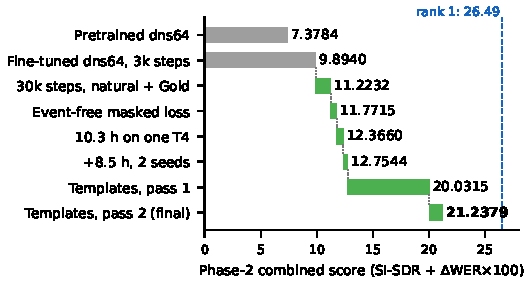
\includegraphics[width=\columnwidth]{fig_bridge.pdf}
\caption{Phase-2 leaderboard combined score after each accepted change (labels: absolute score). Grey: baselines,
each a separate run; green: gain over the previous row. The first green bar compares two separate runs (stage~0
started from the pretrained weights, not from the 3k-step run).}
\label{fig:bridge}
\end{figure}

\begin{table}[t]
\centering
\caption{Ablations on the Phase-2 leaderboard (one submission each)}
\label{tab:abl}
\begin{tabular}{@{}lr@{}}
\toprule
System & Combined \\
\midrule
Pretrained dns64, no fine-tuning$^{a}$ & 7.3784 \\
Fine-tuned 3k steps, natural validation targets & 9.8940 \\
Fine-tuned 6k steps, clean refs as targets, test-like SNR$^{b}$ & 9.0097 \\
Fine-tuned 30k steps, natural + Gold targets (stage 0)$^{c}$ & 11.2232 \\
+ event-free masked loss, clean refs as targets (stage 1) & 11.7715 \\
+ 10.3\,h long run (stage 2) & 12.3660 \\
+ 8.5\,h continuation, 2-seed mean (stage 3) & 12.7544 \\
Stage 2 with ESC-50 noise added to the bank (branch) & 12.0588 \\
Pass-1 subtraction, hit clips not denoised afterwards$^{d}$ & 6.1181 \\
Templates pass 1 + denoiser & 20.0315 \\
\textbf{Templates pass 1+2 + denoiser (final)} & \textbf{21.2379} \\
\bottomrule
\end{tabular}
\par\vspace{2pt}
{\footnotesize\raggedright $^{a}$No unprocessed-input submission; early near-identity submissions scored SI-SDR
7.4--8.2\,dB, so the pretrained model is at input level. $^{b}$From the pretrained weights; test-like SNR
$\approx$7.5\,dB, estimated from those submissions. $^{c}$Differs from the 3k-step row in both steps and targets;
started from the pretrained weights. $^{d}$Other clips keep the stage-3 denoiser output.\par}
\end{table}

Table~\ref{tab:abl} lists the main ablations. Every row is a single submission, so we add per-clip sign tests on the
500 listed clips where we have them (binomial $p<10^{-6}$ for each): stage~0 beats the 3k-step run on 430 clips,
stage~3 beats stage~2 on 459 (+0.18\,dB mean), the ESC-50 branch is worse than stage~2 on 344, and the final system
beats stage~3 on 478; the stage-1 and stage-2 gains were not tested per clip. Subtraction without denoising the hit
clips scores only 6.1181, below the pretrained model: it leaves residue, speech-biased gains, spurious hits,
unmatched noises and alignment error, which the following denoiser largely repairs (6.1181 to 20.0315); the two
steps are complementary. Stage~3's +0.39 mixes longer training and two-seed averaging (single seeds were not
submitted). The clean-reference variant (9.0097) changed three things at once (targets, noise SNR, 6k steps), so
its deficit is not attributed to one cause.

\textbf{Limitations.} Template discovery is transductive: it runs on the test audio itself and exploits a property
of the organisers' generator (a finite noise library), so it is not a general denoising method; its precision and
recall were measured neither on test (no labels) nor on validation, so the over-detection signs in
Sec.~\ref{sec:tpl} are the only evidence on false positives. On recordings with unique noise only the denoiser acts
(the 12.7544-level system). Model selection used the Phase\nobreakdash-2 leaderboard: 20--26 submissions in total
(old submission files were deleted to free Codabench storage, so the exact count is not recoverable); the 12 scores
quoted here (Table~\ref{tab:abl} and the 5.40 run of Sec.~\ref{sec:tpl}) informed design decisions, the rest were
packaging or audit re-uploads and early near-identity variants (outputs close to the inputs). Training-run variance was not estimated (the stage-3 seeds were only averaged).

\textbf{Conclusion.} When a test set is generated from a finite noise library, the noise itself can be recovered
without labels by correlating denoiser residuals across clips. Exact subtraction of the recovered waveforms, then a
learned denoiser, lifted the combined score from 12.7544 to 21.2379, rank~2 (rank~1: 26.4894). The released code,
checkpoints and templates regenerated the 24 test clips we checked bit-identically on our laptop GPU (12 with
template hits); other GPUs may differ in the lowest fp16 bits.

\begin{thebibliography}{9}
\bibitem{vaani} ARTPARK, IISc and Google, ``Vaani noise event dataset,'' Hugging Face,
\url{https://huggingface.co/datasets/ARTPARK-IISc/Vaani-Noise-Event-Dataset}, 2026.
\bibitem{esc50} K.~J.~Piczak, ``ESC: Dataset for environmental sound classification,'' in \emph{Proc. ACM
Multimedia}, 2015.
\bibitem{sisdr} J.~Le~Roux, S.~Wisdom, H.~Erdogan and J.~R.~Hershey, ``SDR -- half-baked or well done?'' in
\emph{Proc. ICASSP}, 2019.
\bibitem{demucs} A.~D\'efossez, G.~Synnaeve and Y.~Adi, ``Real time speech enhancement in the waveform domain,'' in
\emph{Proc. Interspeech}, 2020.
\bibitem{dns} C.~K.~A.~Reddy \emph{et al.}, ``The INTERSPEECH 2020 deep noise suppression challenge: Datasets,
subjective testing framework, and challenge results,'' in \emph{Proc. Interspeech}, 2020.
\bibitem{turin} G.~L.~Turin, ``An introduction to matched filters,'' \emph{IRE Trans. Inf. Theory}, vol.~6, no.~3,
pp.~311--329, 1960.
\bibitem{lewis} J.~P.~Lewis, ``Fast normalized cross-correlation,'' in \emph{Vision Interface}, 1995.
\bibitem{mallat} S.~G.~Mallat and Z.~Zhang, ``Matching pursuits with time-frequency dictionaries,'' \emph{IEEE
Trans. Signal Process.}, vol.~41, no.~12, pp.~3397--3415, 1993.
\bibitem{repet} Z.~Rafii and B.~Pardo, ``REpeating Pattern Extraction Technique (REPET): A simple method for
music/voice separation,'' \emph{IEEE Trans. Audio, Speech, Lang. Process.}, vol.~21, no.~1, pp.~73--84, 2013.
\bibitem{denoiserrepo} Facebook Research, ``denoiser,'' v0.1.5, \url{https://github.com/facebookresearch/denoiser},
2020.
\bibitem{sravaani} ARTPARK-IISc, ``SraVaani-1.0,'' \url{https://huggingface.co/ARTPARK-IISc/SraVaani-1.0}, 2026.
\end{thebibliography}

\end{document}
